\documentclass[a4paper,12pt]{article}
\usepackage[a4paper, top = 1cm, bottom = 1.5cm, left = 1cm, right = 1cm, marginparwidth = 1cm]{geometry}

\usepackage{cmap}					% поиск в PDF
\usepackage[T2A]{fontenc}			% кодировка
\usepackage[utf8]{inputenc}			% кодировка исходного текста
\usepackage[english,russian]{babel}	% локализация и переносы

\usepackage{amsmath}
\usepackage{amssymb}
\usepackage{cancel}
\usepackage{graphicx}
\usepackage{float}
\usepackage{subfig}
\usepackage{tabularx}
\usepackage{longtable}
\usepackage[colorlinks=true, citecolor=red, linkcolor=red, urlcolor=blue]{hyperref}

\DeclareMathOperator\arctanh{arctanh}
\numberwithin{equation}{section}
\title{Второе задание}
\author{
	Хохлов Алексей \\
}

\begin{document}
	\maketitle
	

	%1
	\section{Проекция на шар}
	
	Если $\Vert \mathbf{a} \Vert_2 \leqslant 1$, то, очевидно, проекция $\mathbf{p} = \mathbf{a}$.
	
	Если же $\Vert \mathbf{a} \Vert_2 > 1$, очевидно, что искомая точка --- точка пересечения прямой, соединяющей центр сферы и $\mathbf{a}$, с поверхностью единичной сферы. Другими словами, искомая точка $\mathbf{p} = \dfrac{\mathbf{a}}{\Vert \mathbf{a} \Vert_2 }$. Чтобы доказать это, покажем, что $\forall \mathbf{x} \in \mathbf{X}  $ верно $\Vert \mathbf{a} - \mathbf{x} \Vert_2 \geqslant  \Vert \mathbf{a} - \mathbf{p} \Vert_2$.
	
	Для правой стороны неравенства
	
	\begin{equation}
	\Vert \mathbf{a} - \mathbf{p} \Vert_2 = \Vert \mathbf{a} - \frac{\mathbf{a}}{\Vert \mathbf{a} \Vert_2} \Vert_2 =  ( 1 - \frac{1}{\Vert \mathbf{a} \Vert_2}) \Vert \mathbf{a} \Vert_2  = \Vert \mathbf{a} \Vert_2 - 1
	\end{equation}
	
	Для левой стороны неравенства
	
	\begin{equation}
	\Vert \mathbf{a} - \mathbf{x} \Vert_2 \geqslant \Vert \mathbf{a} \Vert_2 - \Vert \mathbf{x} \Vert_2 \geqslant \Vert \mathbf{a} \Vert_2 - 1 = \Vert \mathbf{a} - \mathbf{p} \Vert_2
	\end{equation}
	
	Видим, что для любой точки в единичном шаре точка $\mathbf{p} = \dfrac{\mathbf{a}}{\Vert \mathbf{a} \Vert_2 }$ является решением задачи
	
	\begin{equation}
	\Vert \mathbf{a} - \mathbf{x} \Vert_2 \rightarrow \text{min}
	\end{equation}
	
	%2
	\section{Минимизация скалярного произведения}
	
	Искомая точка
	
	\begin{align}
	p_i &=
	\left\{
	\begin{aligned}
	1 ,\; & i = k\\
	0 ,\; & i \neq k
	\end{aligned}
	\right. \\
	\end{align}
	
	где $k$ --- такая, что $c_k = \text{min}(c_1, c_2,...,c_n)$. Докажем это.
	
	Поскольку $c_k \leqslant c_i$ для любого $i$, то $c_k x_i \leqslant c_i x_i$. Значит, что
	
	\begin{equation}
	\left\langle \mathbf{c},\mathbf{p} \right\rangle  = c_k = c_k \sum\limits_{i=1}^{n}  x_i =  \sum\limits_{i=1}^{n} c_k x_i \leqslant \sum\limits_{i=1}^{n} c_i x_i = \left\langle \mathbf{c},\mathbf{x} \right\rangle
	\end{equation}
	
	
	%3
	\section{Максимизация функции правдоподобия}
	
	В решении использованы формулы
	
	\begin{equation}
	\label{prove32}
	\frac{\partial}{\partial \mathbf{A}}(\text{tr}(\mathbf{A}^{-1}\mathbf{B})) = -(\mathbf{A}^{-1}\mathbf{B}\mathbf{A}^{-1})^{\text{T}}
	\end{equation}
	
	\begin{equation}
	\label{det31}
	\frac{\partial }{\partial \mathbf{A}} \text{det} (\mathbf{A})= \text{det} (\mathbf{A}) \mathbf{A}^\text{-T}
	\end{equation}
	
	\begin{equation}
	\label{abc}
	\text{tr}(\mathbf{A}\mathbf{B}\mathbf{C}) = \text{tr}(\mathbf{B}\mathbf{C}\mathbf{A})
	\end{equation}
	
	%3.1
	
	
	\subsection{}
	Разложим функцию на слагаемые
	\begin{equation}
	f = \frac{m}{2} \log \text{det} \Sigma + \frac 12 \sum\limits_{i=1}^{m} (\mathbf{x}_i -\boldsymbol{\mu} )^\text{T} \Sigma^{-1} (\mathbf{x}_i -\boldsymbol{\mu} ) = f_1 + f_2
	\end{equation}
	
	Найдем производные слагаемых по $\Sigma$.
	
	Для первого слагаемого воспользуемся~\eqref{det31} 
	
	\begin{equation}
	\frac{\partial}{\partial \Sigma} f_1 = \frac m2 \frac{1}{\text{det}\Sigma} \text{det} (\Sigma) \Sigma^{-\text{T}} = \frac m2 \Sigma^{-\text{T}}
	\end{equation}
	
	Для второго слагаемого воспользуемся~\eqref{abc} и~\eqref{prove32}.
	
	\begin{equation}
	\begin{split}
	&\frac{\partial}{\partial \Sigma}  f_2= \frac 12 \frac{\partial}{\partial \Sigma} \text{tr} (\sum\limits_{i=1}^{m} (\mathbf{x}_i -\boldsymbol{\mu} )^\text{T} \Sigma^{-1} (\mathbf{x}_i -\boldsymbol{\mu} )) = \frac 12 \frac{\partial}{\partial \Sigma} \text{tr} ( \Sigma^{-1}\sum\limits_{i=1}^{m}  (\mathbf{x}_i -\boldsymbol{\mu} ) (\mathbf{x}_i -\boldsymbol{\mu} )^\text{T}) = \\
	& =- \frac 12  \left(  \Sigma^{-1} (\sum\limits_{i=1}^{m}  (\mathbf{x}_i -\boldsymbol{\mu} ) (\mathbf{x}_i -\boldsymbol{\mu} )^\text{T}) \Sigma^{-1}\right) ^\text{T} = - \frac 12  \Sigma^{-T} \left( \sum\limits_{i=1}^{m}  (\mathbf{x}_i -\boldsymbol{\mu} ) (\mathbf{x}_i -\boldsymbol{\mu} )^\text{T}\right)^\text{T}  \Sigma^{-T}
	\end{split}
	\end{equation}
	
	Приравняем производную функции к нулю
	
	\begin{equation}
	\frac m2 \Sigma^{-\text{T}} - \frac 12  \Sigma^{-T} \left( \sum\limits_{i=1}^{m}  (\mathbf{x}_i -\boldsymbol{\mu} ) (\mathbf{x}_i -\boldsymbol{\mu} )^\text{T}\right)^\text{T}  \Sigma^{-T} = 0
	\end{equation}
	
	Умножив на $\Sigma$ и транспонировав, получим
	
	\begin{equation}
	\Sigma = \frac 1m  \sum\limits_{i=1}^{m}  (\mathbf{x}_i -\boldsymbol{\mu} ) (\mathbf{x}_i -\boldsymbol{\mu} )^\text{T}
	\end{equation}
	
	%3.2
	\subsection{}
	
	Докажем формулу~\eqref{prove32}. Во-первых, из $\mathbf{A}\mathbf{A}^{-1} = \mathbf{E}$ следует
	
	\begin{equation}
	\frac{\partial}{\partial a_{pq}} \sum\limits_{j=1}^{n} \tilde{a}_{ij} a_{jk} =  \sum\limits_{j=1}^{n} \frac{\partial \tilde{a}_{ij}}{\partial a_{pq}} a_{jk} + \sum\limits_{j=1}^{n} \tilde{a}_{ij}  \frac{\partial a_{jk}}{\partial a_{pq}} = 0
	\end{equation}
	
	Домножая справа на обратную матрицу, получим
	
	\begin{equation}
	\label{inverse_derivative}
	\frac{\partial \tilde{a}_{ij}}{\partial a_{pq}} = - \sum\limits_{k=1}^{n} \sum\limits_{m=1}^{n} \tilde{a}_{im}  \frac{\partial a_{mk}}{\partial a_{pq}} \tilde{a}_{kj}  = - \tilde{a}_{ip}  \tilde{a}_{qj} 
	\end{equation}
	
	Раскроем теперь производную следа
	
	\begin{equation}
	\frac{\partial}{\partial a_{pq}}(\text{tr}(\mathbf{A}^{-1}\mathbf{B})) = \frac{\partial}{\partial a_{pq}} \sum\limits_{i=1}^{n} \sum\limits_{j=1}^{n} \tilde{a}_{ij} b_{ji} = \sum\limits_{i=1}^{n} \sum\limits_{j=1}^{n} \frac{\partial \tilde{a}_{ij}}{\partial a_{pq}} b_{ji}
	\end{equation}
	
	Подставляя значение производной из~\eqref{inverse_derivative}
	
	\begin{equation}
	\frac{\partial}{\partial a_{pq}}(\text{tr}(\mathbf{A}^{-1}\mathbf{B})) = - \sum\limits_{i=1}^{n} \sum\limits_{j=1}^{n} \tilde{a}_{ip}  \tilde{a}_{qj}  b_{ji} =  - \sum\limits_{i=1}^{n} \sum\limits_{j=1}^{n} \tilde{a}_{pi}^\text{T} b_{ij}^\text{T}  \tilde{a}_{jq}^\text{T} 
	\end{equation}
	
	получим в матричном виде искомую формулу~\eqref{prove32}.
	%4
	\section{Парабола}
	$(x-3)(x-1) \leqslant 0$ --- задача оптимизации решается на множестве $Q = \left[ 1;3\right] $
	
	%4a
	\subsection{a}
	
	$\dfrac{\partial}{\partial x}(x^2+1)=2x > 0$, $\dfrac{\partial^2}{\partial x^2}(x^2+1)=1 > 0$ --- функция строго возрастающая на отрезке $\left[1;3\right]$. Значит, минимальное значение достигается в точке $x=1$.
	
	\begin{equation}
	\min_{x \in Q} (x^2+1) = x^2+1|_{x=1}=2
	\end{equation}
	%4b
	\subsection{b}
	\begin{figure}[H]
		\center{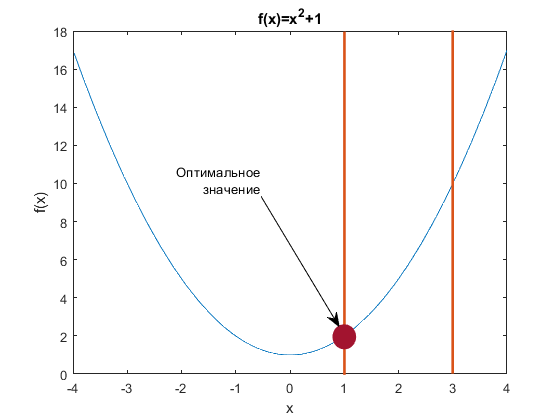
\includegraphics[width=0.8\textwidth]{./4b.png}}\\
		\caption{Целевая функция, допустимое множество и оптимальное значение.}
	\end{figure}
	%4c
	\subsection{c}
	\begin{equation}
	L(x, \mu) = x^2+1 + \mu(x-1)(x-3) = (1+\mu)x^2 - 4 \mu x + (1+3\mu)
	\end{equation}
	
	Лагранжиан --- параболическая функция. При $\mu <= -1$ инфинум $\inf L = -\infty$. При $\mu > -1$ минимум параболического лагранжиана достигается в точке $x = \dfrac{2\mu}{(1+\mu)}$. Двойственная функция запишется так:
	
	\begin{equation}
	g(\mu) = \inf L(x, \mu) = \frac{4\mu^2}{1+\mu} - \frac{8\mu^2}{1+\mu} + \frac{(1+3\mu)(1+\mu)}{1+\mu} = \frac{-\mu^2 + 4\mu +1}{1+\mu} = -\mu + 5 - \frac{4}{1+\mu} 
	\end{equation}
	
	\begin{figure}[H]
		\center{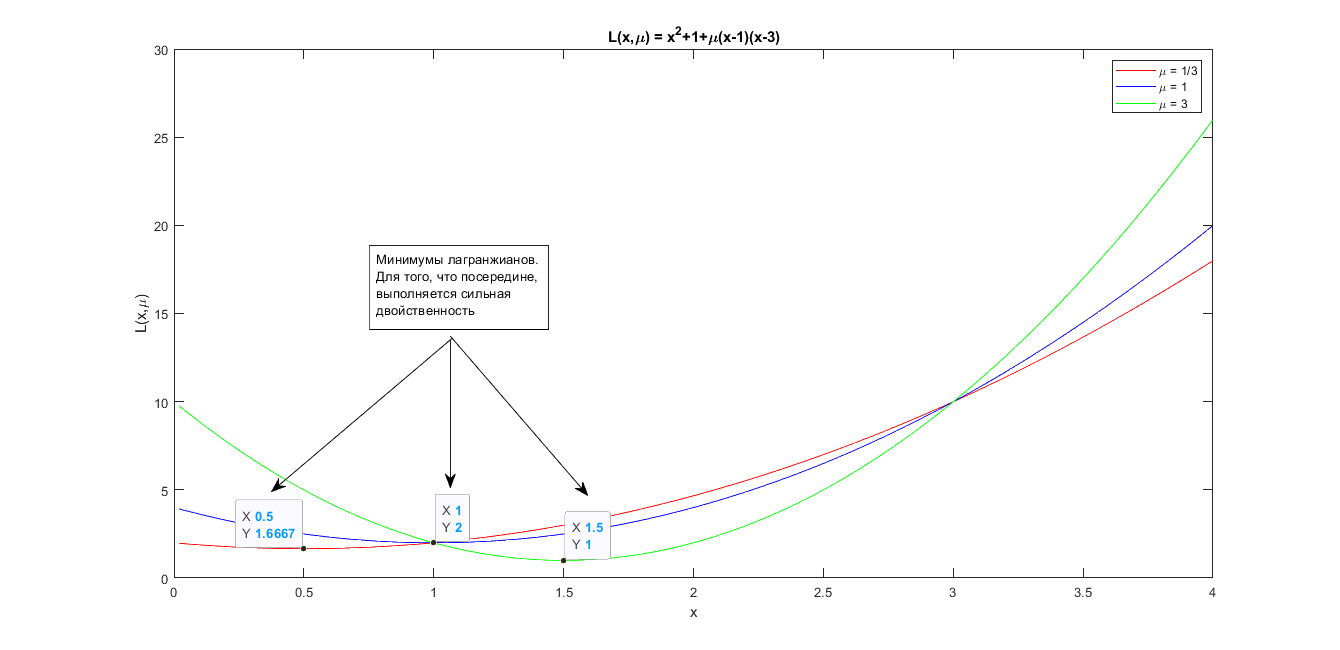
\includegraphics[width=1.0\textwidth]{./44.png}}\\
		\caption{График лагранжиана для нескольких	$\mu$. $p^{*} \geqslant \inf_{x} L(x, \mu)$}
	\end{figure}
	

	
	%4d
	\subsection{d}
	Формулировка двойственной задачи:
	
	\begin{align}
	\begin{aligned}
	&\max g(\mu) = \max (-\mu + 5 - \frac{4}{1+\mu})  \\
	&\text{s.t.}\mu \geqslant 0
	\end{aligned}
	\end{align}
	
	Найдем первую и вторую производные двойственной функции:
	
	\begin{equation}
	\frac{\partial}{\partial \mu} g(\mu) = -1 + \frac{4}{(1+\mu)^2}
	\end{equation}
	
	\begin{equation}
	\frac{\partial^2}{\partial \mu^2} g(\mu) = -\frac{8}{(1+\mu)^3}
	\end{equation}
	
	При $\mu \geqslant 0$, как видно, двойственная функция является вогнутой, и поэтому ее экстремум при $\mu = 1$ является максимумом.
	
	\begin{equation}
	\max_{\mu \geqslant 0} g(\mu) = g(\mu)|_{\mu=1} = 2 = (x^2+1)|_{x=1} =\min_{x \in Q} (x^2+1)
	\end{equation}
	
	Сильная двойственность выполняется.
	
	%5
	\section{Задача бинарного линейного программирования}
	
	%5.1
	\subsection{}
	
	Задачу можно переписать в виде
	
	\begin{align}
	\begin{aligned}
	&\min_{\mathbf{x}} \mathbf{c}^{\text{T}}\mathbf{x} \\
	&x_i(x_i-1) = 0, i= 1,...,n\\
	&\mathbf{A}\mathbf{x} \leqslant \mathbf{b}
	\end{aligned}
	\end{align}
	
	Лагранжиан запишется в виде
	
	\begin{align}
	&L(\mathbf{x},\boldsymbol{\lambda},\boldsymbol{\mu}) = \sum\limits_{i=1}^{n}\left( c_i x_i + \lambda_i x_i(x_i-1)\right) + \sum\limits_{j}\mu_j (\sum\limits_{j=1}^{n}a_{ji}x_i - b_j) = \\
	&= \sum\limits_{i=1}^{n} \left(\lambda_i x_i^2 + \left[ c_i-\lambda_i + \sum\limits_{j}\mu_j a_{ji}\right] x_i \right)  + \sum\limits_{j}\mu_j b_j
	\end{align}
	
	Лагранжиан --- параболическая функция. Рассмотрим лагранжиан при разных параметрах.
	
	Если найдется такая $i$,что $\lambda_i < 0$, то инфинум $\inf L = -\infty$. 
	
	Если найдется такая $i$,что $\lambda_i = 0, c_i + \sum_j \mu_j a_{ji} \neq 0$, то инфинум $\inf L = -\infty$.  
	
	Пусть теперь либо $\lambda_i = 0, c_i + \sum_j \mu_j a_{ji} \ = 0$, либо $\lambda_i > 0$. Если для $i$ выполнено первое условие, то вклад в инфинум функции от слагаемых, соответвующих этим $i$, равен нулю. Слагаемые, для которых выполнено второе условие, достигают минимума в точке $x_i = -\dfrac{ c_i-\lambda_i + \sum\limits_{j}\mu_j a_{ji}}{2\lambda_i}$
	
	Инфинум запишется в виде
	
	\begin{equation}
	\label{5doublefunc}
	g(\boldsymbol{\lambda},\boldsymbol{\mu}) = \inf_x L = -\sum_i \frac{\left(  c_i-\lambda_i + \sum\limits_{j}\mu_j a_{ji}\right)^2 }{4\lambda_i} + \sum_j \mu_j b_j
	\end{equation}
	
	Суммирование ведется по таким $i$, что $\lambda_i > 0$.
	

	%5.2
	\subsection{}
	
	Задача для непрерывной релаксации перепишется следующим образом:
	
	\begin{align}
	\begin{aligned}
	&\min_{\mathbf{x}} \mathbf{c}^{\text{T}}\mathbf{x} \\
	&x_i(x_i-1) \leqslant 0, i= 1,...,n\\
	&\mathbf{A}\mathbf{x} \leqslant \mathbf{b}
	\end{aligned}
	\end{align}
	
	Видно, что двойственная функция $g(\boldsymbol{\mu},\boldsymbol{\tilde{\mu}})$ запишется в таком же виде, что и в~\eqref{5doublefunc}, только $\tilde{\mu}_i$ вместо $\lambda_i$, причём для $\tilde{\mu}_i$ условие $\tilde{\mu}_i \geqslant 0$ будет автоматически выполнено при поиске решения двойственной задачи. Соответственно, при $\lambda_i \geqslant 0$ максимумы двойственных функций совпадут друг с другом, и, иными словами, нижняя оценка релаксации Лагранжа совпадет с оценкой непрерывной релаксации.
	
	Поскольку выполняются условия ККТ, то решение этой задачи действительно дает оценку снизу.
	
	
	
	%6
	\section{Задача наименьших квадратов}
	
	\subsection{}
	Лагранжиан для задачи запишется так:
	\begin{equation}
	L(\mathbf{x},\boldsymbol{\lambda}) = \frac 12 \Vert \mathbf{A}\mathbf{x}-\mathbf{b} \Vert_2^2 +\boldsymbol{\lambda}^{\text{T}} (\mathbf{G}\mathbf{x}-\textbf{h}) 
	\end{equation}
	
	Производная лагранжиана по $\mathbf{x}$ такова 
	
	\begin{equation}
	\frac{\partial}{\partial \mathbf{x}}L(\mathbf{x},\boldsymbol{\lambda}) = \mathbf{A}^{\text{T}}(\mathbf{A}\mathbf{x}-\mathbf{b}) +\mathbf{G}^{\text{T}}\boldsymbol{\lambda} = \mathbf{A}^{\text{T}}\mathbf{A}\mathbf{x}-(\mathbf{A}^{\text{T}}\mathbf{b} -\mathbf{G}^{\text{T}}\boldsymbol{\lambda})
	\end{equation}
	
	С одной стороны, по теореме о ранге произведения матриц, ранг матрицы $\mathbf{A}^{\text{T}}\mathbf{A}$ не превосходит $n$. С другой стороны, по неравенству Сильвестра $2n = \text{rank}(\mathbf{A}^{\text{T}}) + \text{rank}(\mathbf{A}) \leqslant \text{rank}(\mathbf{A}^{\text{T}}\mathbf{A}) + n$. Итак, ранг матрицы($n\times n$) $\mathbf{A}^{\text{T}}\mathbf{A}$ равен $n$ --- значит, для неё существует обратная.
	
	Тогда $\dfrac{\partial}{\partial \mathbf{x}}L(\mathbf{x}^{*},\boldsymbol{\lambda}) = 0$ при $\mathbf{x}^{*} =(\mathbf{A}^{\text{T}}\mathbf{A})^{-1}(\mathbf{A}^{\text{T}}\mathbf{b} -\mathbf{G}^{\text{T}}\boldsymbol{\lambda})$. Отсюда можно получить двойственную функцию. 
	
	Двойственная задача запишется так:
	
	\begin{equation}
	\max_{\mathbf{\lambda}} \frac 12 \Vert \mathbf{A}(\mathbf{A}^{\text{T}}\mathbf{A})^{-1}(\mathbf{A}^{\text{T}}\mathbf{b} -\mathbf{G}^{\text{T}}\boldsymbol{\lambda})-\mathbf{b} \Vert_2^2 +\boldsymbol{\lambda}^{\text{T}} \left( \mathbf{G}(\mathbf{A}^{\text{T}}\mathbf{A})^{-1}(\mathbf{A}^{\text{T}}\mathbf{b} -\mathbf{G}^{\text{T}}\boldsymbol{\lambda})-\textbf{h}\right) 
	\end{equation}
	
	Для исходной (выпуклой) задачи выполнены условия ККТ --- значит, выполняется сильная двойственность, т.е. решение двойственной задачи совпадает с решением исходной.
	 
	\subsection{}
	
	 Найдём решение исходной задачи. Подставим найденное $\mathbf{x}^{*}$ в равенство $\mathbf{G}\mathbf{x}=\mathbf{h}$. Получим
	
	\begin{equation}
	\mathbf{G}(\mathbf{A}^{\text{T}}\mathbf{A})^{-1}(\mathbf{A}^{\text{T}}\mathbf{b} -\mathbf{G}^{\text{T}}\boldsymbol{\lambda}^{*}) = \mathbf{h}
	\end{equation}
	
	\begin{equation}
	\mathbf{G}(\mathbf{A}^{\text{T}}\mathbf{A})^{-1}\mathbf{A}^{\text{T}}\mathbf{b} - \mathbf{h}=\mathbf{G}(\mathbf{A}^{\text{T}}\mathbf{A})^{-1}\mathbf{G}^{\text{T}}\boldsymbol{\lambda}^{*}
	\end{equation}
	
	Матрица перед $\boldsymbol{\lambda}^{*}$ представляет собой произведение трех матриц: $\mathbf{G}$ размера $p\times n$ и ранга $p$, $(\mathbf{A}^{\text{T}}\mathbf{A})^{-1}$ размера $n\times n$ и ранга $n$, $\mathbf{G}^{\text{T}}$ размера $n\times p$ и ранга $p$. Итоговая матрица имеет размер $p \times p$. Если $p \leqslant n$, то применяя теорему о ранге произведения и неравенство Сильвестра, получим, что ранг итоговой матрицы($p \times p$) равен $p$ --- она обратима. Тогда решение исходной задачи запишется как
	
	\begin{equation}
	\boldsymbol{\lambda}^{*} =\left[ \mathbf{G}(\mathbf{A}^{\text{T}}\mathbf{A})^{-1}\mathbf{G}^{\text{T}}\right] ^{-1} \left[\mathbf{G}(\mathbf{A}^{\text{T}}\mathbf{A})^{-1}\mathbf{A}^{\text{T}}\mathbf{b} - \mathbf{h} \right] 
	\end{equation}
	
	\begin{equation}
	\mathbf{x}^{*} =(\mathbf{A}^{\text{T}}\mathbf{A})^{-1}(\mathbf{A}^{\text{T}}\mathbf{b} -\mathbf{G}^{\text{T}}\boldsymbol{\lambda}^{*})
	\end{equation}
	
	\begin{equation}
	\min_{\mathbf{x}} f(\mathbf{x}) = \frac 12 \Vert \mathbf{A}\mathbf{x}^{*}-\mathbf{b} \Vert_2^2 =  g(\boldsymbol{\lambda}^{*})=\max_{\boldsymbol{\lambda}} g(\boldsymbol{\lambda})
	\end{equation}
	
	%7
	\section{Условие на матрицу}
	
	\subsection{}

	Из критерия Сильвестра (все главные миноры неотрицательны) равносильная запись задачи
	
	\begin{equation}
	\begin{split}
	&\text{min}( y_1)\\
	\text{s.t.}&y_2 \geqslant 0\\
	&y_1+1 \geqslant 0\\
	&y_2(y_1+1) \geqslant 0\\
	-&y_1^2(y_1+1) \geqslant 0\\
	-&y_1^2 \geqslant 0
	\end{split}
	\end{equation}
	
	Или в каноничной записи
	
	 \begin{equation}
	 \begin{split}
	 &\text{min}( y_1)\\
	 \text{s.t.}&-y_2 \leqslant 0\\
	 -&y_1-1 \leqslant 0\\
	 -&y_2(y_1+1) \leqslant 0\\
	 &y_1^2(y_1+1) \leqslant 0\\
	 &y_1^2 \leqslant 0
	 \end{split}
	 \end{equation}
	 
	В такой записи задача не является выпуклой, т.к. функция $y_1^2(y_1+1)$ является выпуклой не при всех $\mathbf{y}$.
	 
	Упростим условия:
	
	\begin{equation}
	\begin{split}
	&\text{min} (y_1)\\
	\text{s.t.}&y_2 \geqslant 0\\
	&y_1 = 0\\
	\end{split}
	\end{equation}
	
	Решение - $y_1 = 0$, $y_2 \geqslant 0$
	
	\subsection{}
		
	Лагранжиан можно записать как
	
	\begin{equation}
	\begin{split}
	&L(y_1,y_2, \Lambda) = y_1 - \text{tr}(\mathbf{Y}^{\text{T}}\mathbf{\Lambda}) = y_1 -  y_1\lambda_{21} - y_1\lambda_{12} - y_2\lambda_{22} - (y_1+1)\lambda_{33} =\\
	 & = y_1 (1 -  \lambda_{21} - \lambda_{12} - \lambda_{33} )- \lambda_{22} y_2 - \lambda_{33} 
	\end{split}
	\end{equation}
	
	$\mathbf{\mathbf{Y}^{\text{T}}\mathbf{\Lambda}} =\left( \begin{matrix}
	 & 0 & y_1 & 0 \\
	 & y_1 & y_2 & 0 \\
	 & 0 & 0 & y_1 +1 
	\end{matrix}\right) 
	\left( \begin{matrix}
	& \lambda_{11} & \lambda_{12} & \lambda_{13} \\
	& \lambda_{21} & \lambda_{22} & \lambda_{23} \\
	& \lambda_{31} & \lambda_{32} & \lambda_{33} 
	\end{matrix}\right) = 	
	\left( \begin{matrix}
	& y_1\lambda_{21} & ... & ... \\
	& ... & y_1\lambda_{12}+y_2\lambda_{22} & ... \\
	& ... & ... & (y_1+1)\lambda_{33} 
	\end{matrix}\right)  $
	
	\begin{align}
	\begin{aligned}
	&\dfrac{\partial}{\partial y_1} L(y_1,y_2, \Lambda) =  1 -  \lambda_{21} - \lambda_{12} - \lambda_{33} = 0 \\
	&\dfrac{\partial}{\partial y_2} L(y_1,y_2, \Lambda) = - \lambda_{22} = 0 
	\end{aligned}
	\end{align}
	
	Отсюда
	
	\begin{equation}
	 L(y_1,y_2, \Lambda) = -\lambda_{33}
	\end{equation}
	
	Для двойственной задачи 

	\begin{align}
	\inf_{y_1,y_2} L &=
	\left\{
	\begin{aligned}
	-\infty ,\; & \lambda_{22} \neq 0, 1 -  \lambda_{21} - \lambda_{12} - \lambda_{33} \neq 0\\
	-\lambda_{33} ,\;  &\lambda_{22} = 0, 1 -  \lambda_{21} - \lambda_{12} - \lambda_{33} = 0
	\end{aligned}
	\right. \\
	\end{align}
	
	\begin{equation}
	\max g(\Lambda) = \max (-\lambda_{33}) = +\infty
	\end{equation}
	
	Зазор двойственности --- $+\infty$. Сильная двойственность не выполняется, т.к. не выполняется условие неотрицательности $\Lambda$ при оптимальных двойственных переменных.
		
\end{document}

